% ============================================================================
% Section 8: Network Protocol
% ============================================================================

\section{Network Protocol}
\label{sec:network}

\Botho employs a peer-to-peer network protocol optimized for privacy
transaction propagation and consensus message delivery.

\subsection{Network Architecture}

\subsubsection{Node Types}

\begin{itemize}
  \item \textbf{Full nodes}: Store complete blockchain, validate all
    transactions, participate in consensus
  \item \textbf{Minting nodes}: Full nodes that additionally perform PoW
    and propose blocks
  \item \textbf{Light clients}: Store block headers only, verify
    transactions via inclusion proofs
\end{itemize}

% Node Type Hierarchy Diagram
% Shows different node types and their capabilities
%
% ACCESSIBILITY ALT TEXT:
% A vertical hierarchy diagram showing three node types. Top: Minting Node
% (orange box) - block producer with PoW and SCP participation, requires
% 200+ GB storage and 16 GB RAM. Middle: Full Node (blue box) - validator
% with complete blockchain storage and transaction validation, requires 100+
% GB and 8 GB RAM. Bottom: Light Client (green box) - wallet with headers
% only and SPV proofs, requires minimal resources. Dashed arrows show
% inheritance (Full extends to Minting) and trust (Light trusts Full).
% Left brace indicates decreasing trust requirements from top to bottom.

\begin{figure}[ht]
\centering
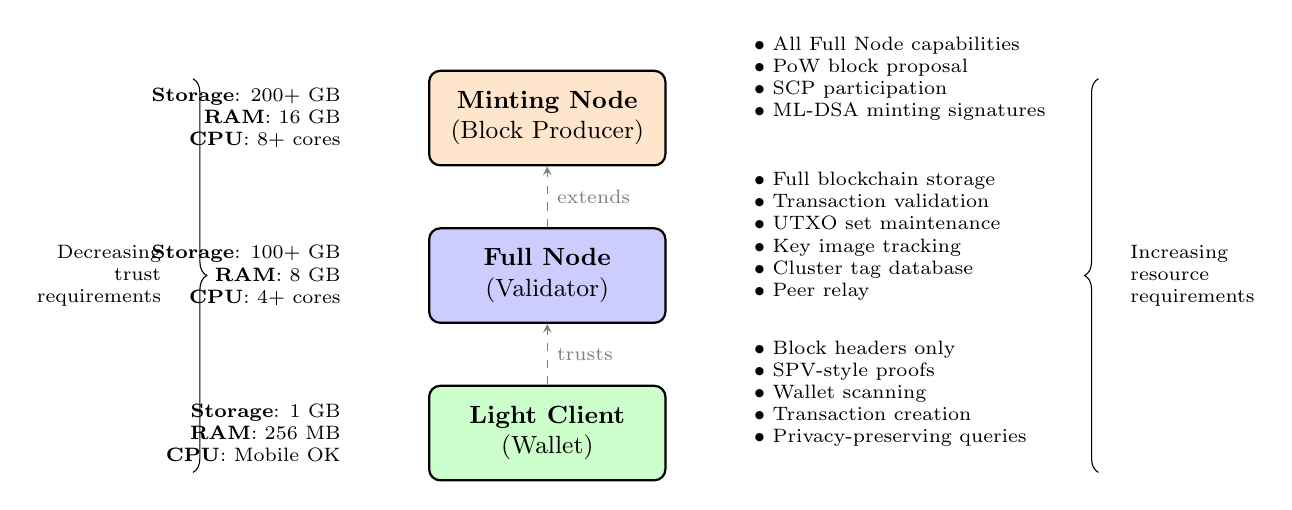
\begin{tikzpicture}[
    node distance=1cm,
    nodetype/.style={rectangle, draw, rounded corners, minimum width=3cm, minimum height=1.2cm, align=center, font=\small},
    full/.style={nodetype, fill=blue!20, thick},
    minting/.style={nodetype, fill=orange!20, thick},
    light/.style={nodetype, fill=green!20, thick},
    capability/.style={font=\scriptsize, align=left},
    arrow/.style={->, >=stealth, thick},
    inherit/.style={->, >=stealth, dashed, gray},
]

% Node types (arranged in hierarchy)
\node[minting] (minting) at (0,4) {\textbf{Minting Node}\\(Block Producer)};
\node[full] (full) at (0,2) {\textbf{Full Node}\\(Validator)};
\node[light] (light) at (0,0) {\textbf{Light Client}\\(Wallet)};

% Inheritance arrows
\draw[inherit] (full) -- (minting) node[midway, right, font=\scriptsize] {extends};
\draw[inherit] (light) -- (full) node[midway, right, font=\scriptsize] {trusts};

% Capabilities for Minting Node
\node[capability, anchor=west] at (2.5,4.5) {
    $\bullet$ All Full Node capabilities\\
    $\bullet$ PoW block proposal\\
    $\bullet$ SCP participation\\
    $\bullet$ ML-DSA minting signatures
};

% Capabilities for Full Node
\node[capability, anchor=west] at (2.5,2.5) {
    $\bullet$ Full blockchain storage\\
    $\bullet$ Transaction validation\\
    $\bullet$ UTXO set maintenance\\
    $\bullet$ Key image tracking\\
    $\bullet$ Cluster tag database\\
    $\bullet$ Peer relay
};

% Capabilities for Light Client
\node[capability, anchor=west] at (2.5,0.5) {
    $\bullet$ Block headers only\\
    $\bullet$ SPV-style proofs\\
    $\bullet$ Wallet scanning\\
    $\bullet$ Transaction creation\\
    $\bullet$ Privacy-preserving queries
};

% Storage requirements (left side)
\node[font=\scriptsize, anchor=east, align=right] at (-2.5,4) {
    \textbf{Storage}: 200+ GB\\
    \textbf{RAM}: 16 GB\\
    \textbf{CPU}: 8+ cores
};

\node[font=\scriptsize, anchor=east, align=right] at (-2.5,2) {
    \textbf{Storage}: 100+ GB\\
    \textbf{RAM}: 8 GB\\
    \textbf{CPU}: 4+ cores
};

\node[font=\scriptsize, anchor=east, align=right] at (-2.5,0) {
    \textbf{Storage}: 1 GB\\
    \textbf{RAM}: 256 MB\\
    \textbf{CPU}: Mobile OK
};

% Trust model annotation
\draw[decorate, decoration={brace, amplitude=5pt, mirror}]
    (-4.5,-0.5) -- (-4.5,4.5)
    node[midway, left=8pt, font=\scriptsize, align=right] {
        Decreasing\\
        trust\\
        requirements
    };

\draw[decorate, decoration={brace, amplitude=5pt}]
    (7,-0.5) -- (7,4.5)
    node[midway, right=8pt, font=\scriptsize, align=left] {
        Increasing\\
        resource\\
        requirements
    };

\end{tikzpicture}
\caption{Node type hierarchy in \Botho. Light clients trust full nodes for
transaction validation but verify headers independently. Full nodes maintain
complete state and validate all transactions. Minting nodes extend full nodes
with block proposal capabilities. Resource requirements scale with trust
assumptions---light clients trade some security for accessibility.}
\label{fig:node-hierarchy}
\end{figure}


\subsubsection{Transport Layer}

All peer-to-peer communication uses:
\begin{itemize}
  \item \textbf{TCP}: Reliable delivery for consensus messages
  \item \textbf{Noise Protocol}~\cite{noise}: Authenticated encryption
    with forward secrecy
  \item \textbf{Multiplexed streams}: Separate channels for different
    message types
\end{itemize}

\subsection{Peer Discovery}

\subsubsection{Bootstrap Nodes}

New nodes connect to hardcoded bootstrap nodes to discover initial peers:

\begin{lstlisting}[language=,caption={Bootstrap node configuration}]
BootstrapNodes {
    dns_seeds: [
        "seed1.botho.org",
        "seed2.botho.org",
        "seed3.botho.org",
    ],
    static_peers: [
        "203.0.113.1:9732",
        "203.0.113.2:9732",
    ],
}
\end{lstlisting}

\subsubsection{Kademlia DHT}

Peer discovery uses a modified Kademlia DHT~\cite{kademlia}:

\begin{itemize}
  \item Node IDs derived from public keys (not chosen)
  \item XOR distance metric for routing
  \item Iterative lookup with parallel queries
  \item Periodic bucket refresh
\end{itemize}

\subsubsection{Peer Limits}

\begin{table}[h]
\centering
\caption{Connection limits}
\label{tab:peer-limits}
\begin{tabular}{@{}lc@{}}
\toprule
\textbf{Category} & \textbf{Limit} \\
\midrule
Outbound connections & 8 \\
Inbound connections & 117 \\
Total connections & 125 \\
Connections per IP & 2 \\
\bottomrule
\end{tabular}
\end{table}

\subsection{Message Protocol}

\subsubsection{Message Types}

\begin{lstlisting}[language=,caption={Message enumeration}]
enum Message {
    // Handshake
    Hello { version, genesis_hash, best_height },
    HelloAck { version, genesis_hash, best_height },

    // Block propagation
    NewBlock { block },
    GetBlocks { locator, stop_hash },
    Blocks { blocks },

    // Transaction propagation
    NewTransaction { tx },
    GetTransactions { hashes },
    Transactions { txs },

    // Consensus (SCP)
    SCPNomination { msg },
    SCPPrepare { msg },
    SCPCommit { msg },
    SCPExternalize { msg },

    // Compact blocks
    CompactBlock { header, short_ids },
    GetBlockTxs { block_hash, indices },
    BlockTxs { block_hash, txs },
}
\end{lstlisting}

\subsubsection{Message Serialization}

Messages are serialized using a canonical binary format:
\begin{itemize}
  \item Little-endian byte order
  \item Varint encoding for lengths
  \item No padding or alignment
  \item Deterministic ordering of map keys
\end{itemize}

\subsubsection{Wire Format Specification}

Each message follows the structure:

\begin{lstlisting}[caption={Message wire format}]
Message {
    magic: [u8; 4],        // Network identifier: 0x00 0x0B 0x07 0xB0
    type_id: u8,           // Message type discriminant
    length: varint,        // Payload length in bytes
    checksum: [u8; 4],     // First 4 bytes of SHA256(payload)
    payload: [u8; length], // Type-specific data
}
\end{lstlisting}

\textbf{Message type identifiers}:

\begin{table}[h]
\centering
\caption{Message type encoding}
\label{tab:msg-types}
\begin{tabular}{@{}clc@{}}
\toprule
\textbf{ID} & \textbf{Message} & \textbf{Max Size} \\
\midrule
0x00 & Hello & 256 B \\
0x01 & HelloAck & 256 B \\
0x10 & NewBlock & 2 MB \\
0x11 & GetBlocks & 4 KB \\
0x12 & Blocks & 10 MB \\
0x20 & NewTransaction & 100 KB \\
0x21 & GetTransactions & 4 KB \\
0x22 & Transactions & 1 MB \\
0x30 & SCPNomination & 64 KB \\
0x31 & SCPPrepare & 64 KB \\
0x32 & SCPCommit & 64 KB \\
0x33 & SCPExternalize & 64 KB \\
0x40 & CompactBlock & 64 KB \\
0x41 & GetBlockTxs & 4 KB \\
0x42 & BlockTxs & 1 MB \\
0xFF & Ping/Pong & 8 B \\
\bottomrule
\end{tabular}
\end{table}

\textbf{Field-level encoding}:

\begin{lstlisting}[caption={Common field encodings}]
// Varint: 7 bits per byte, MSB = continuation
fn encode_varint(n: u64) -> Vec<u8> {
    let mut bytes = Vec::new();
    let mut value = n;
    while value >= 0x80 {
        bytes.push((value & 0x7F) | 0x80);
        value >>= 7;
    }
    bytes.push(value as u8);
    bytes
}

// Hash: 32 bytes, raw
Hash = [u8; 32]

// CompressedPoint: 32 bytes (Ristretto255)
Point = [u8; 32]

// Signature: Variable (CLSAG ~700B, ML-DSA ~3.3KB)
Signature = varint(len) ++ [u8; len]

// Block header: Fixed 120 bytes
BlockHeader {
    version: u8,             // 1 byte
    prev_hash: [u8; 32],     // 32 bytes
    merkle_root: [u8; 32],   // 32 bytes
    timestamp: u64,          // 8 bytes (little-endian)
    height: u64,             // 8 bytes
    difficulty: u64,         // 8 bytes
    nonce: u64,              // 8 bytes
    minter_key_hash: [u8; 32], // 32 bytes
}
\end{lstlisting}

\subsection{Protocol State Machine}

\subsubsection{Connection States}

Each peer connection transitions through defined states:

\begin{lstlisting}[caption={Connection state machine}]
enum ConnectionState {
    Connecting,      // TCP handshake in progress
    Authenticating,  // Noise protocol handshake
    Handshaking,     // Hello/HelloAck exchange
    Active,          // Normal operation
    Syncing,         // Initial block download
    Stale,           // No activity timeout
    Disconnecting,   // Graceful shutdown
}

// State transitions
Connecting     -> Authenticating  [TCP established]
Authenticating -> Handshaking     [Noise complete]
Handshaking    -> Active          [HelloAck received, compatible]
Handshaking    -> Disconnecting   [Incompatible version/genesis]
Active         -> Syncing         [Peer ahead by >10 blocks]
Syncing        -> Active          [Caught up]
Active         -> Stale           [No messages for 5 minutes]
Stale          -> Active          [Pong received]
Stale          -> Disconnecting   [No Pong after 30 seconds]
*              -> Disconnecting   [Error or ban]
\end{lstlisting}

\subsubsection{Message Sequences}

\textbf{Connection establishment}:
\begin{enumerate}
  \item Initiator: TCP connect to peer:9732
  \item Both: Noise XX handshake (mutual authentication)
  \item Initiator: Send Hello \{version, genesis\_hash, best\_height\}
  \item Responder: Send HelloAck (if compatible) or disconnect
  \item Both: Transition to Active state
\end{enumerate}

\textbf{Block synchronization}:
\begin{enumerate}
  \item Node A: Send GetBlocks \{locator, stop\_hash\}
  \item Node B: Find common ancestor from locator
  \item Node B: Send Blocks \{blocks[ancestor+1..min(ancestor+500, stop)]\}
  \item Node A: Validate and apply blocks
  \item Node A: Repeat from step 1 if more blocks needed
\end{enumerate}

\textbf{Transaction relay}:
\begin{enumerate}
  \item Sender: Receive transaction (local or from peer)
  \item Sender: Validate transaction fully
  \item If in stem phase: Forward to single stem peer
  \item If in fluff phase: Announce via NewTransaction to all peers
  \item Receivers: Request full transaction if not in mempool
  \item Receivers: Validate and continue relay
\end{enumerate}

\textbf{Consensus message flow}:
\begin{enumerate}
  \item Proposer: Broadcast NewBlock upon PoW solution
  \item Validators: Validate block, enter nomination
  \item Validators: Exchange SCPNomination messages
  \item Validators: Upon nomination convergence, send SCPPrepare
  \item Validators: Upon prepare quorum, send SCPCommit
  \item Validators: Upon commit quorum, send SCPExternalize
  \item All nodes: Apply externalized block as final
\end{enumerate}

\subsubsection{Error Handling}

Protocol errors trigger specific responses:

\begin{table}[h]
\centering
\caption{Protocol error handling}
\label{tab:error-handling}
\begin{tabular}{@{}lll@{}}
\toprule
\textbf{Error} & \textbf{Action} & \textbf{Score Penalty} \\
\midrule
Invalid checksum & Drop message & -1 \\
Unknown message type & Drop message & 0 \\
Message too large & Drop + warn & -10 \\
Invalid block header & Drop block & -50 \\
Invalid transaction & Drop tx & -10 \\
Invalid signature & Drop + ban & -1000 \\
Rate limit exceeded & Throttle & -5/excess \\
Protocol violation & Disconnect & -1000 \\
\bottomrule
\end{tabular}
\end{table}

\textbf{Reconnection policy}:
\begin{itemize}
  \item Disconnected peers: Retry after exponential backoff (1s, 2s, 4s, ..., 1h max)
  \item Banned peers: No reconnection for 24 hours
  \item Repeated bans: Permanent blacklist after 3 bans
\end{itemize}

\subsection{Block Propagation}

\subsubsection{Compact Block Relay}

To reduce bandwidth, blocks are relayed in compact form:

\begin{enumerate}
  \item Sender transmits compact block (header + short transaction IDs)
  \item Receiver reconstructs from mempool
  \item Receiver requests missing transactions by index
  \item Sender provides requested transactions
\end{enumerate}

\textbf{Short ID computation}:
\begin{equation}
\text{short\_id} = \text{SipHash}(\text{nonce} \| \text{txid})_{[0:6]}
\end{equation}

Average bandwidth savings: 90\% (most transactions already in mempool).

\subsubsection{Block Validation}

Upon receiving a block:
\begin{enumerate}
  \item Validate header (PoW, timestamp, difficulty)
  \item Verify Merkle root
  \item Validate each transaction
  \item Verify minting transaction signature
  \item Verify SCP proof (quorum agreement)
  \item Apply to local state
\end{enumerate}

\subsection{Transaction Propagation}

\subsubsection{Dandelion++}

Transaction propagation uses Dandelion++~\cite{dandelion} to protect
sender network identity:

\textbf{Stem phase}:
\begin{itemize}
  \item Transaction relayed along a random path
  \item Each hop has probability $p$ to switch to fluff phase
  \item Path length follows geometric distribution
\end{itemize}

\textbf{Fluff phase}:
\begin{itemize}
  \item Standard flooding to all peers
  \item Cannot trace back to stem origin
\end{itemize}

% Dandelion++ Propagation Diagram
% Shows stem phase (linear) transitioning to fluff phase (broadcast)
%
% ACCESSIBILITY ALT TEXT:
% A network diagram showing transaction propagation in two phases. Left
% (Stem Phase): A red origin node connects linearly through orange relay
% nodes S1, S2, S3 - hiding the true source. Right (Fluff Phase): After
% probabilistic transition, a green fluff source broadcasts to multiple
% blue nodes F1-F9 in a tree pattern. Legend explains that adversaries
% observing the fluff phase cannot determine the true origin, providing
% network-level privacy with plausible deniability.

\begin{figure}[ht]
\centering
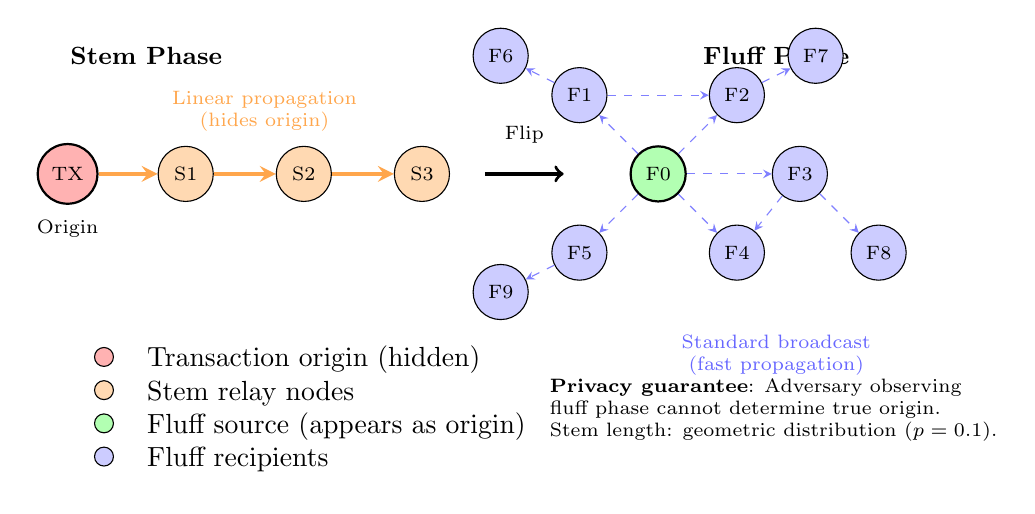
\begin{tikzpicture}[
    node distance=1.2cm,
    peer/.style={circle, draw, minimum size=0.7cm, font=\scriptsize},
    origin/.style={peer, fill=red!30, thick},
    stem/.style={peer, fill=orange!30},
    fluff/.style={peer, fill=blue!20},
    stempath/.style={->, >=stealth, thick, orange!70, line width=1.5pt},
    fluffpath/.style={->, >=stealth, dashed, blue!50},
    label/.style={font=\small\bfseries},
]

% === Stem Phase (left side) ===
\node[label] at (-4,3) {Stem Phase};

% Origin node
\node[origin] (o) at (-5,1.5) {TX};
\node[font=\scriptsize] at (-5,0.8) {Origin};

% Stem path nodes
\node[stem] (s1) at (-3.5,1.5) {S1};
\node[stem] (s2) at (-2,1.5) {S2};
\node[stem] (s3) at (-0.5,1.5) {S3};

% Stem arrows
\draw[stempath] (o) -- (s1);
\draw[stempath] (s1) -- (s2);
\draw[stempath] (s2) -- (s3);

% Stem annotation
\node[font=\scriptsize, align=center, orange!70] at (-2.5,2.3) {
    Linear propagation\\
    (hides origin)
};

% Transition marker
\draw[very thick, ->] (0.3,1.5) -- (1.3,1.5);
\node[font=\scriptsize] at (0.8,2) {Flip};

% === Fluff Phase (right side) ===
\node[label] at (4,3) {Fluff Phase};

% Fluff source (last stem node becomes fluff source)
\node[fluff, thick, fill=green!30] (f0) at (2.5,1.5) {F0};

% First ring of fluff nodes
\node[fluff] (f1) at (1.5,2.5) {F1};
\node[fluff] (f2) at (3.5,2.5) {F2};
\node[fluff] (f3) at (4.3,1.5) {F3};
\node[fluff] (f4) at (3.5,0.5) {F4};
\node[fluff] (f5) at (1.5,0.5) {F5};

% Second ring
\node[fluff] (f6) at (0.5,3) {F6};
\node[fluff] (f7) at (4.5,3) {F7};
\node[fluff] (f8) at (5.3,0.5) {F8};
\node[fluff] (f9) at (0.5,0) {F9};

% Fluff arrows from center
\draw[fluffpath] (f0) -- (f1);
\draw[fluffpath] (f0) -- (f2);
\draw[fluffpath] (f0) -- (f3);
\draw[fluffpath] (f0) -- (f4);
\draw[fluffpath] (f0) -- (f5);

% Fluff arrows from first ring
\draw[fluffpath] (f1) -- (f6);
\draw[fluffpath] (f2) -- (f7);
\draw[fluffpath] (f3) -- (f8);
\draw[fluffpath] (f5) -- (f9);

% Cross-connections in fluff
\draw[fluffpath] (f1) -- (f2);
\draw[fluffpath] (f3) -- (f4);

% Fluff annotation
\node[font=\scriptsize, align=center, blue!60] at (4,-0.8) {
    Standard broadcast\\
    (fast propagation)
};

% === Legend and explanation ===
\node[anchor=west] at (-5,-1.5) {
    \begin{tabular}{cl}
    \tikz\draw[fill=red!30, draw] (0,0) circle (0.12); & Transaction origin (hidden) \\
    \tikz\draw[fill=orange!30, draw] (0,0) circle (0.12); & Stem relay nodes \\
    \tikz\draw[fill=green!30, draw] (0,0) circle (0.12); & Fluff source (appears as origin) \\
    \tikz\draw[fill=blue!20, draw] (0,0) circle (0.12); & Fluff recipients \\
    \end{tabular}
};

% Privacy note
\node[align=left, font=\scriptsize, anchor=west] at (1,-1.5) {
    \textbf{Privacy guarantee}: Adversary observing\\
    fluff phase cannot determine true origin.\\
    Stem length: geometric distribution ($p = 0.1$).
};

\end{tikzpicture}
\caption{Dandelion++ transaction propagation~\cite{dandelion}. In the \textit{stem phase},
transactions propagate along a random linear path, obscuring the origin. After
a probabilistic transition (average 10 hops), the \textit{fluff phase} begins:
standard broadcast propagation for fast network-wide dissemination. The fluff
source appears to be the transaction origin, providing plausible deniability
for the true sender.}
\label{fig:dandelion}
\end{figure}


\subsubsection{Transaction Validation}

Transactions are validated before relay:
\begin{enumerate}
  \item Syntactic validity (correct encoding)
  \item Semantic validity (signatures verify)
  \item Contextual validity (references exist, no double-spend)
  \item Fee sufficiency
\end{enumerate}

Invalid transactions are dropped; peers sending invalid transactions are
deprioritized.

\subsection{Synchronization}

\subsubsection{Initial Block Download}

New nodes synchronize via:
\begin{enumerate}
  \item Connect to peers and exchange best heights
  \item Download block headers (verify PoW chain)
  \item Request blocks in parallel from multiple peers
  \item Validate and apply blocks sequentially
  \item Join consensus once synchronized
\end{enumerate}

\subsubsection{Block Locator}

Block requests include a locator to identify common ancestor:

\begin{lstlisting}[language=,caption={Block locator construction}]
fn block_locator(tip: Height) -> Vec<Hash> {
    let mut locator = Vec::new();
    let mut step = 1;
    let mut height = tip;

    while height > 0 {
        locator.push(hash_at(height));
        if locator.len() > 10 {
            step *= 2;
        }
        height = height.saturating_sub(step);
    }
    locator.push(genesis_hash());
    locator
}
\end{lstlisting}

This logarithmic structure efficiently identifies divergence point.

\subsubsection{Pruning}

Full nodes may prune old blocks while retaining:
\begin{itemize}
  \item Recent blocks (configurable, default 10,000)
  \item Block headers (all)
  \item UTXO set (current state)
  \item Key image set (all, for double-spend detection)
\end{itemize}

Pruned nodes cannot serve historical blocks but can fully validate new
transactions.

\subsection{Denial-of-Service Protection}

\subsubsection{Rate Limiting}

Per-peer rate limits:
\begin{itemize}
  \item Block requests: 10/second
  \item Transaction announcements: 100/second
  \item Consensus messages: 50/second
\end{itemize}

\subsubsection{Peer Scoring}

Peers maintain reputation scores:
\begin{itemize}
  \item +1 for valid blocks/transactions
  \item -10 for invalid data
  \item -100 for protocol violations
  \item Disconnect at score $<$ -1000
\end{itemize}

\subsubsection{Resource Bounds}

\begin{itemize}
  \item Maximum message size: 100 KB
  \item Maximum block size: 2 MB
  \item Maximum mempool size: 100 MB
  \item Maximum pending requests: 1000
\end{itemize}

\subsection{Privacy Considerations}

\subsubsection{Traffic Analysis Resistance}

\begin{itemize}
  \item \textbf{Dandelion++}: Hides transaction origin
  \item \textbf{Encrypted transport}: Prevents content inspection
  \item \textbf{No timing correlation}: Messages are batched and jittered
\end{itemize}

\subsubsection{Tor/I2P Support}

Optional routing through anonymity networks:
\begin{itemize}
  \item Tor hidden service support
  \item I2P integration planned
  \item Mixed clearnet/onion peer connections
\end{itemize}

\subsection{Light Client Security}
\label{sec:light-clients}

Light clients enable mobile and resource-constrained devices to participate
in the network with reduced trust assumptions compared to custodial solutions.

\subsubsection{Verification Capabilities}

Light clients can verify:
\begin{itemize}
  \item \textbf{Transaction inclusion}: Merkle proofs demonstrate transaction
    is in a specific block
  \item \textbf{Block header chain}: PoW verification confirms work was expended
  \item \textbf{SCP finality}: Externalization proofs confirm consensus agreement
  \item \textbf{Output ownership}: Local key derivation identifies owned outputs
\end{itemize}

Light clients \emph{cannot} verify:
\begin{itemize}
  \item \textbf{Transaction validity}: Ring signature verification requires
    full UTXO context
  \item \textbf{Double-spend prevention}: Requires complete key image database
  \item \textbf{Value conservation}: Commitment arithmetic needs all inputs
\end{itemize}

\subsubsection{Trust Model}

Light clients trust full nodes for:

\begin{enumerate}
  \item \textbf{Transaction validity}: Full nodes could relay invalid
    transactions (mitigated by connecting to multiple independent nodes)
  \item \textbf{Completeness}: Full nodes could withhold transactions
    (mitigated by querying multiple nodes)
  \item \textbf{Privacy}: Query patterns reveal interest (mitigated by
    fetching broader data ranges)
\end{enumerate}

\textbf{Security level}: Comparable to SPV in Bitcoin---economically secure
against profit-motivated attackers but vulnerable to targeted attacks by
well-resourced adversaries.

\subsubsection{Output Scanning}

Light clients scan for received funds:

\begin{lstlisting}[caption={Light client scanning protocol}]
LightClientScan {
    // Request outputs in block range
    GetOutputs {
        start_height: u64,
        end_height: u64,
    },

    // Response: encrypted output data
    Outputs {
        outputs: Vec<(Height, TxIndex, EncryptedOutput)>,
    },
}
\end{lstlisting}

For each output, the client:
\begin{enumerate}
  \item Attempts ML-KEM decapsulation with view key
  \item If successful, derives one-time key and checks match
  \item Decrypts amount if output belongs to wallet
\end{enumerate}

\textbf{Privacy consideration}: Downloading all outputs in a range (rather
than requesting specific ones) prevents servers from learning which outputs
the client owns.

\subsubsection{Transaction Submission}

Light clients construct transactions locally:
\begin{enumerate}
  \item Select ring members from cached output set
  \item Build transaction with local keys (never transmitted)
  \item Submit to multiple full nodes via Dandelion++ stem
\end{enumerate}

\textbf{Ring member selection}: Light clients maintain a local cache of
recent outputs sufficient for ring construction. This cache is populated
during scanning and can be refreshed from any full node.

\subsubsection{Privacy Implications}

Light client operations leak information:

\begin{table}[h]
\centering
\caption{Light client information leakage}
\label{tab:light-privacy}
\begin{tabular}{@{}ll@{}}
\toprule
\textbf{Operation} & \textbf{Information Leaked} \\
\midrule
Block header sync & Active time periods \\
Output scanning & Block ranges of interest \\
Ring member fetch & Potential transaction construction \\
TX submission & Approximate location (IP-based) \\
\bottomrule
\end{tabular}
\end{table}

\textbf{Mitigation strategies}:
\begin{itemize}
  \item Connect via Tor/I2P for IP privacy
  \item Scan broader ranges than necessary
  \item Cache ring members proactively
  \item Submit transactions to random nodes
\end{itemize}

\subsubsection{Comparison to Full Node Security}

\begin{table}[h]
\centering
\caption{Full node vs. light client security}
\label{tab:node-comparison}
\begin{tabular}{@{}lcc@{}}
\toprule
\textbf{Property} & \textbf{Full Node} & \textbf{Light Client} \\
\midrule
Validate all transactions & Yes & No \\
Detect double-spends & Yes & No \\
Verify consensus & Yes & Partial \\
Independent operation & Yes & No \\
Receive funds securely & Yes & Yes* \\
Send funds securely & Yes & Yes \\
Privacy (network) & High & Medium \\
\bottomrule
\end{tabular}
\end{table}

\textit{*Light clients can verify they received funds but must trust that
the sending transaction was valid.}

\subsubsection{Mobile Wallet Recommendations}

For mobile deployments:
\begin{itemize}
  \item Use light client with multiple independent servers
  \item Prefer Tor connections when available
  \item Cache sufficient outputs for offline transaction construction
  \item Verify transaction inclusion before considering funds confirmed
  \item Consider running personal full node as trusted backend
\end{itemize}

\subsection{Network Constants}

\begin{table}[h]
\centering
\caption{Network protocol constants}
\label{tab:network-constants}
\begin{tabular}{@{}lrl@{}}
\toprule
\textbf{Parameter} & \textbf{Value} & \textbf{Description} \\
\midrule
Default port & 9732 & Main network \\
Testnet port & 19732 & Test network \\
Protocol version & 1 & Current version \\
Magic bytes & \texttt{0xB07B0} & Network identifier \\
Handshake timeout & 10s & Connection setup \\
Ping interval & 60s & Keepalive \\
\bottomrule
\end{tabular}
\end{table}

